\documentclass{amsart}
\usepackage{graphicx}
\graphicspath{{./}}
\usepackage{hyperref}
\usepackage{csvsimple}
\usepackage{longtable}
\usepackage{lscape}
\usepackage{epigraph}
\title{Discrete Correlation of Human Race Measurements}
\author{Zulfikar Moinuddin Ahmed}
\date{\today}
\begin{document}
\maketitle

\section{Summary}

We introduce discrete correlations of categorical variables that are valid for the first time as a metric in statistics.  No measure had existed that is valid for evaluating strength of relationships.  We give complete R code for our discrete correlation metric.

Then we present the calculation of the discrete correlation matrix for some data from World Values Survey 7 using $n=510$ columns.  We examine the eigenvalues of the $100 \times 100$ correlation matrix and assess the fit of the eigenvalue distribution by a Generalised Hyperbolic Distribution.  We consider this distribution to be a universal quantity that allows us to formulate a coherent full scientific theory of Human Nature that is quantitative.



\section{Code}

\begin{verbatim}
# Zulf's Proportional Chi-Square

prop.chisq<-function( data ){
  m<-dim(data)[1]
  n<-dim(data)[2]
  t<-0
  v0<-data[1,]/sum(data[1,])
  for (j in 2:m){
    v<-data[j,]/sum(data[j,])
    t<- t + sum( (v-v0)^2/v0^2)
  }
  df<-1
  t0<-qchisq(0.95, df=df)
  pval <- 1 - pchisq( t, df=df)
  list(tstat=t,pval=pval,crit=t0)
}


g<-function(x){
  #print(x)
  log(-log(x)+0.01)
}

zulf.sigma<-function(z){
  n<-length(z)
  if (n==1){
    return(1)
  }
  #print(n)
  D<-matrix(0, nrow=n, ncol=n)
  diag(D)<-1
  #print(dim(D))
  s<-0
  for (j in 2:n){
    for (k in 1:j){
      gg = abs(z[j] - z[k])
      D[j,k] <- gg
      D[k,j] <- gg
      s<-s + gg
    }
  }
  out<- 2*s/(n^2-n)
  out
}

zulf.chisq<-function( data ){
  data<-as.matrix(data)
  m<-dim(data)[1]
  n<-dim(data)[2]
  if ( m<=1 || n<=1){
    return(list(tstat=0,pval=1,t0=1))
  }
  t<-0
  eps<-0.00001
  w0 <- (data[1,]+eps)/sum(data[1,]+eps)
  #print('this')
  #print(length(w0))
  
  v0<- log(-log(abs(w0)+eps))
  #print(v0)
  sigma0 <- zulf.sigma( v0 )
  mu0 <- mean(v0)
  for (j in 2:m){
    w<-(data[j,]+eps)/sum(data[j,]+eps)
    #print(w)
    v<-g(w)
    #print('works')
    #print(v)
    #print('---')
    sigma <- zulf.sigma( v )
    mu <- mean(v)
    z <- v/sigma
    z0 <- v0/sigma0
    t<- t + sum( ( z - z0 )^2)
  }
  df<-(n-1)*(m-1)
  t0<-qchisq(0.95, df=df)
  pval <- 1 - pchisq( t, df=df)
  list(tstat=t,pval=pval,crit=t0)
}


# calculate the discrete correlation
# matrix of WVS7
tablify<-function(a, b){
  H<-na.omit(data.frame(a,b))
  T<-matrix(1,nrow=1,ncol=1)
  tryCatch( { T<-table(H) } )
  T
}

cor.d<-function( data ){
  n<-dim(data)[2]
  out<-matrix(0,nrow=n, ncol=n)
  diag(out)<-1
  if (n==2){
    out[1,1]<-1
    out[2,2]<-1
    a<-data[,1]
    b<-data[,2]
    X<-tablify( a, b )
    metrics <- zulf.chisq(X)
    out[1,2] <- 1 - metrics$pval
    out[2,1] <- 1 - metrics$pval
  }
  
  if (n>2){
    for (j in 2:n){
      for (k in 1:j ){
        print(paste(j,k))
        a<-data[,j]
        b<-data[,k]
        X<-tablify( a, b )
        metrics <- zulf.chisq(X)
        print('ok')
        out[j,k] <- 1 - metrics$pval
        out[k,j] <- 1 - metrics$pval
      }
    }
  }
  out
}
\end{verbatim}

\section{Distribution of 100 correlation Eigenvalues}

First let us take a look at the histogram of eigenvalues and the Generalised Hyperbolic Distribution fit.

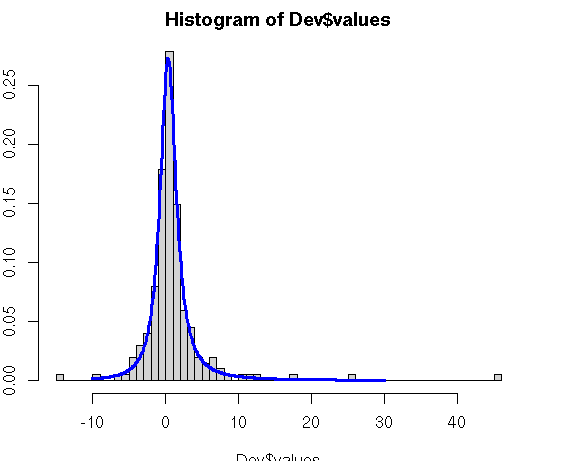
\includegraphics[scale=0.8]{human_values_correl_hist.jpeg}

The Generalised Hyperbolic Fit is quite gorgeous and accurate.

Let's look at the fitted parameters.

\begin{verbatim}
Asymmetric Generalized Hyperbolic Distribution:

Parameters:
      lambda    alpha.bar           mu        sigma 
-0.734819351  0.003937837  0.300662297  8.962769977 
       gamma 
 2.746209012 

Call:
fit.ghypuv(data = Dev$values)

Optimization information:
log-Likelihood:                -480.6028 
AIC:                           971.2055 
Fitted parameters:             lambda, alpha.bar, mu, sigma, gamma;  (Number: 5)
Number of iterations:          294 
Converged:                     TRUE 
\end{verbatim}


\section{Generalised Hyperbolic Distribution Parameters For Human Values Correlation are Scientific Parameters for Human Nature}

We have obtained values with 100 Human Nature Variables.  It is our view that as the number of variables tend to infinity, there will be a convergence to finite parameters of a GHD, and these parameters are {\em Human Nature Invariants}.  This is one of the most important observations in the entire history of Social Science, and one of the greatest scientific discoveries in all of Human History.  This discovery tells us that a smooth parametric distribution describes the empirical distribution of eigenvalues of correlation of {\em every possible human nature measurement at all} in the infinite variable limit. 

\section{What is New here}

I had found that using ordinary correlations, a result of this type exists.  Unfortunately ordinary correlations are meaningless for categorical variables. Here we are presenting a result that is far more significant as science, for {\em discrete correlation} had to be invented and computed for this distribution, and these are valid scientifically for correlation eigenvalues.

\end{document}